% section 5
% Kota Miura (miura@embl.de)

\section{Analysis of Time Series }
\label{sec:timeseries}

In this section, we learn how to analyze dynamics using image sequences.
A time series of digital images, usually called
"stack", contains temporal dynamics of
position and intensity, and kinetics can be obtained from these data.
In general there are three types of dynamics.

\begin{enumerate}
\item Position does not change but intensity changes over time. 
\item Position changes but the intensity does not change. 
\item Both Position and Intensity change over time. 
\end{enumerate}

An example of type (1) is the measurement of cargo transport dynamics in
vesicle trafficking \citep{hirschbergJCB1998}. Transition of protein
localization from ER to Golgi then to the plasma membrane was measured
over time by measuring the signal intensity in each statically
positioned compartment. This type of technique has evolved to various
sophisticated methods based on the same principle -measurement of
signal intensity at a constant position. Type (2) corresponds to the
measurement of movement, or object tracking, and an example is the
single particle tracking of membrane surface proteins \citep{muraseBJ2004}. An example of type (3) measurement is the measurement of
chemotaxis-related protein accumulation dynamics during the
\textit{Dictyostelium} cell migration \citep{Dormann2002}. Analysis
of type (3) dynamics is more specific and advanced, so refer to other
literature \citep{miuraABEB2005}.

\subsection{Importing Image Sequence}

Image sequences captured through microscopes in most cases consists of
multiple of single image frames with numbering (\textit{e.g.} image0001.tif, image0002.tif, image0003.tif\ldots). By
importing such files, we can create a window called
"stack". Image stacks are said to be "3D" because there are three
dimensions, x and y axes, and either z axis or time (in the following,
we abbreviate the former as "x-y-z" and the latter as "x-y-t"). 

Stacks could be saved as a single file. The file header will contain the
information on number of frames that the image contains. This number
will be automatically detected when the stack is opened next time, and
reproduces the stack again. When the sequence is a time series of
three-dimensional stacks, the dimension size of the file is four, and
there are two different ways on how the files are stacked: (1) xy -- z
-- t or (2) xy -- t -- z. The order we see common is (1) but in some
cases you might find out that the order is in (2). If you need to
change the order from one to the other, you could use
"HyperVolume Shuffler" plugin to
change the order. In dimensions above three, there no information is
kept within the file about how the file is ordered. One must know it by
keeping a note separately, or decide the order by going through the
sequence. 

HyperVolumeShuffler Plugin\\
\url{http://rsb.info.nih.gov/ij/plugins/hypervolume-shuffler.html}

Dimension could be even higher. When there are multiple channels with 4D
image, say channel 1 (ch1) and 2 (ch2) each for different labels within
a same cell, then the file is 5D. There could be many possibilities in
the order of the file but this could also be sorted using the
HyperVolumeShuffler PlugIn. 


\begin{indentexercise}{1}
Import multiple files as an image stack.
\ijmenu{[File > Import > Image Sequence\ldots]} will open a dialog window and you must specify the
first file of the image series. Select sample sequence
\textbf{eg5\_spindle\_50000.tif\ldots} Then another dialog window
pops up (Fig. \ref{fig:img129}). 

%figure
\begin{figure}[H]
\begin{center}
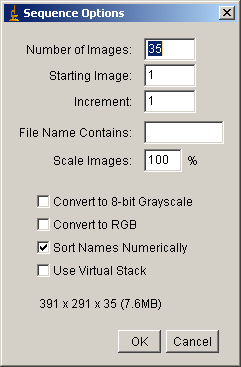
\includegraphics[width=4.657cm,height=7.091cm]{img/CMCIBasicCourse201102-img129.png}
\caption{ Importing multiple frames as a Stack}
\label{fig:img129}
\end{center}
\end{figure}

ImageJ automatically detects the number of files in the folder, and then
another window opens to ask for the number of images you want to
import, which number you want to start with, increment between the
numbering of the file, and also part of the name that is unchanged
through out all the files you want to import. There are other options
such as scaling and conversion of the image but-depth, but these
operations could be also done afterwards. The imported image sequence
is within one window, or a stack.
\end{indentexercise}

Don't close the stack, exercise continues. 

\begin{indentexercise}{2}
In the ImageJ tool bar, there is an icon >> at the right most position. 
Click and from drop down menu, select "Stack tools". 
Video player-like interface appears in the tool bar (\ref{fig:img130}). 
Try different buttons. 
In addition to playback icon button, \ijmenu{[Image > Stacks > Start Animation]} will also play back the movie. 
Try changing the playback speed by \ijmenu{[Image > Stack > Animation options]} (Fig. \ref{fig:img131}). 
%figure
\begin{figure}[htbp]
\begin{center}
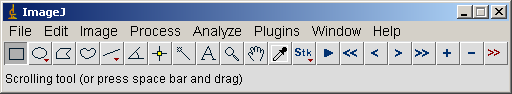
\includegraphics[width=10cm]{img/CMCIBasicCourse201102-img130.png}
\caption{ ImageJ tool bar in Stack Tool mode.}
\label{fig:img130}
\end{center}
\end{figure}

%figure
\begin{figure}[hbtp]
\begin{center}
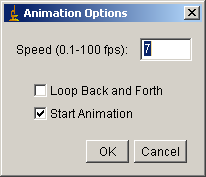
\includegraphics[width=5.45cm,height=4.683cm]{img/CMCIBasicCourse201102-img131.png}
\caption{ Animation Option Window}
\label{fig:img131}
\end{center}
\end{figure}
\end{indentexercise}

\subsection{Difference Images}

In many cases, mathematical manipulation on image sequences is effective
in visualizing dynamics. "Difference images" (also called "subtraction images") is one of such techniques.
A difference image of successive frames in a sequence is given by:
\begin{equation}
D_{j}(x,y)=I_{j+1}(x,y) - I_{j}(x,y)
\end{equation}
where D is the difference image, and j is a given plane in the stack.
Difference images highlight features of the image that change rapidly
over time, much in the same way that a spatial gradient enhances
contrast around an edge. The change is usually brought about by
movement of an object in the image, or by a kinetic process that has
not reached steady-state (like photobleaching).

\begin{indentexercise}{1}
Open image stack \textbf{1703-2(3s-20s).stk}.
Then duplicate the stack \ijmenu{[Edit > Duplicate]}.
Don't forget checking the "Duplicate entire stack". 
Go back to the original stack, delete the last frame (frame 31) \ijmenu{[Image > Stacks >Delete Slice]}. Alternatively, you could simply click "-" button in the stack tools at the last frame. 
Activate the duplicated stack and delete the first frame.
Then do subtraction \ijmenu{[Process > Image > Calculator]}:

\tab $Original Stack - Dupicated Stack$

This will then subtract frame 1 -- frame2, frame2 -- frame 3 \ldots
and so on. Do you see Frapped Region in the difference image stack?
\end{indentexercise}

\subsection{Projections}

A maximum intensity projection of an entire image stack is given by

\begin{equation}
M(x,y) =max_{j}(I_{j}(x,y))
\end{equation}

The maximum on the right hand side is the maximum in intensity value at
a given pixel position over all stacks in an image. Maximum
projections collapse the entire dynamics of the stack onto a single
plane. This function is especially useful for visualizing entire
trajectories of moving particles on a single plane.

\begin{indentexercise}{1}
Open image \textbf{listeriacells.stk}. 
Then do all types of projections you could choose by \ijmenu{[Image > Stack > Z projection\ldots]}.\\
\textbf{Question}: Which is the best method for leaving the bacteria tracks? 
\end{indentexercise}

\subsection{Measurement of Intensity dynamics}

Temporal changes in fluorescence level matters a lot in biological
experiments since the change is directly related to the molecular
mobility and production. Here, we study how to obtain the intensity
dynamics out of image sequences.

\begin{indentexercise}{1}
Load image stack \textbf{1703-2(3s-20s).stk}. 
Make a ROI (could be any closed ROI) at the area where the photobleaching will take place. 
Then do \ijmenu{[Image > Stacks > Plot z-axis Profile]}. 

There will be two windows: "Results" window and a graph of intensity dynamics. 

Try adding Second ROI to measure the background, simply by making another ROI. So the intensity measurement again with this new ROI. 

\textbf{OPTIONAL:} Numerical values in the table can be copy and pasted in spread sheet software like Excel or OpenOffice Calc. Try draw a graph in your favorite plotting software.
\end{indentexercise}

When you measure the fluorescence level, it is necessary to measure the
baseline intensity and subtract the value from the measured
fluorescence. This is because the baseline level adds offset to the
measured value.

\subsection{Measurement of Movement Dynamics}

Movement is an essential component of biological system. To quantify the
movement dynamics, various methods has been developed. In case of image
sequences, particle tracking is a popular way to quantify movement
(\ref{subsubsec:manualtracker}, \ref{subsubsec:autotracker}). 
In any tracking methods, the ultimate goal is to obtain
the position coordinate of a target object in each image frame, so that
the movement of the target object can be represented as changes in the
position coordinate. Velocity and movement direction can then be
calculated from the resulting coordinate series. Since tracking deals
with segmentation and position linking, the process is rather complex.
Besides tracking, there is a easier way to represent and quantify
movements occurring in sequences. The technique is called
"kymographs (\ref{subsubsec:kymograph}: see below)".
This method loses positional information but for measuring velocity,
the method is easy and fast. \\ 

The process of tracking has two major steps. In the first step the
object must be segmented. This then enables us to calculate the
coordinate of the object position, such as its centroid. There are
various ways to do segmentation (see \ref{sec:segmentation}). 
In the second step the successive positions of the object must be linked to obtain a series of
coordinates of that object. We call this process "position linking". Position linking
becomes difficult when there are too many similar objects. In this case
it would become impossible to identify the object in the next time
point among multiple candidates. Position linking also becomes
difficult when the successive positions of the object are too far
apart. This happens when the time interval between frames is too long.
In this case, multiple candidates may appear in the next time point
even though similar objects are only sparsely present in the image
frame. If the target object is single and unique, linking of
coordinates to successive time points has none of these problems. 


\subsection{Kymographs }
\label{subsubsec:kymograph}

Kymographs are a two-dimensional time traces, where time \textit{t} is in Y axis and space along a one-dimensional contour is in \textit{X}, and the dynamical variable \textit{F(x,t) }is
visualized as an image. Kymographs provide a fast and convenient way to
visualize motion and dynamics in microscopy images.

\begin{indentexercise}{1}

Measurement of speed using Kymographs. For doing this exercise, you need "Slice Remover" PlugIn \footnote{ To install the plugin refer to \ref{app1.5}}. 

(1) Load the image stack of a spindle labeled with speckle amounts of tubulin. Name of the file is \textbf{control\_1.stk}. Observe the movie. Note that the tubulin speckles flux towards the both spindle
poles. One way to measure the rate of flux is to create a kymograph along a straight line that runs from one spindle pole to the other.

(2) Remove initial 28 slices by \ijmenu{[plugins > course > Slice Removal]} (Fig. \ref{fig:img132}).

%figure
\begin{figure}[H]
\begin{center}
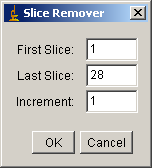
\includegraphics[width=2.778cm,height=3.069cm]{img/CMCIBasicCourse201102-img132.png}
\caption{ Slice Removal dialog}
\label{fig:img132}
\end{center}
\end{figure}


(3) Contrast enhance, and then convert to 8-bit. Then do maximum intensity Z-projection \ijmenu{[Image > Stacks > Z-projection]}. 

Choose segmented line ROI tool (should right click to choose). Then trace one of the tracks in the projection image (Fig. \ref{fig:img133}).

%figure
\begin{figure}[htbp]
\begin{center}
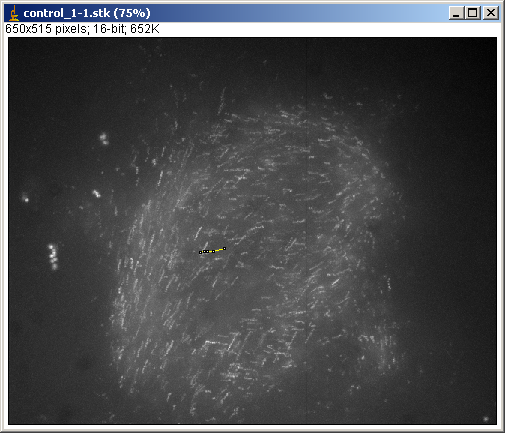
\includegraphics[width=8cm]{img/CMCIBasicCourse201102-img133.png}
\caption{ Tracing Projected Image. Note Small Yellow Segmented ROI in the middle of the image.}
\label{fig:img133}
\end{center}
\end{figure}

Go back to the stack, \ijmenu{[Edit > Selection > Restore Selection]}. Then \ijmenu{[Image > Stacks > Reslice\ldots]}. Don"t change parameters in the dialog window, simply OK. In the kymograph you just now generated, use straight line ROI tool to make a selection along diagonal bright signal (Fig. \ref{fig:img134}). 

%figure
\begin{figure}[htbp]
\begin{center}
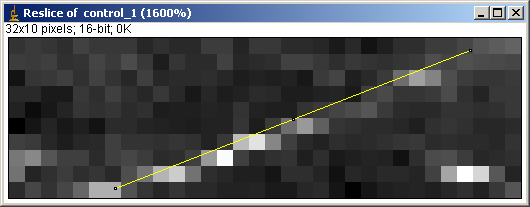
\includegraphics[width=8.467cm,height=3.307cm]{img/CMCIBasicCourse201102-img134.png}
\caption{ Measurement of Kymograph}
\label{fig:img134}
\end{center}
\end{figure}

Install macro "K\_read\_kymoLineROI.txt" by \ijmenu{[PlugIns > Macros >Install\ldots]} and then select the macro file in file chooser, and click OK. Do \ijmenu{[PlugIns > Macros > Show Line
Coordinates and Speed]}. Results will appear in the Log window. 

Note: Jens Rietdorf and Arne Seitz made a Kymograph plug-in for ImageJ. It enables multiple ROI selections, to make your life easier. \\
\url{http://www.embl.de/eamnet/html/kymograph.html}

\end{indentexercise}

\subsection{Manual Tracking}
\label{subsubsec:manualtracker}

In the simplest case, tracking can be done manually. The user can read
out the coordinate position of the target object directly from the
imaging software. In ImageJ, user can read out position coordinate
indicated in the status bar by placing the cross-hair pointer over the
object. Then coordinates can be listed in standard spreadsheet software
such as Microsoft Excel for further analysis. 

An ImageJ plug-in is also freely available to assist such simple way of
tracking. An obvious disadvantage of the manual tracking is that the
mouse-clicking by the user could be erroneous, as we are still human
who gets tired after thousands of clicking. For such errors,
measurement errors can be estimated by tracking the same object several
times and this error could then be indicated together with the results.
Otherwise, automated tracking is more objective, but if you have only
limited number of tracks to analyze, manual tracking is a best choice
before start to explore complex parameter space of automated tracking
setting.

The manual tracking can be assisted by an ImageJ plug-in
"Manual Tracking". This plug-in
enables the user to record x-y coordinates of the position where the
user clicked using mouse in each frame within a stack. The download
site has a detailed instruction on how to use.  


\url{http://rsb.info.nih.gov/ij/plugins/track/track.html}


\begin{indentexercise}{1}
\label{exer:manualtracking}
\item Manual Tracking: In a spindle, microtubules attach to chromosomes through structures called kinetochores. In the stack \textbf{kin.stk}, kinetochores are labeled with a fluorescent marker. Your task now is to track the movement of individual kinetochores using the ManualTracker PlugIn. Enhance contrast and convert the image stack from 16-bit to 8-bit (just to decrease the memory load. If your computer is powerful enough, you don't need to downgrade the stack). Then do \ijmenu{[Plugins > Course > Manual Tracking]}: a window pops up (Fig. \ref{fig:img135}). 

%figure
\begin{figure}[H]
\begin{center}
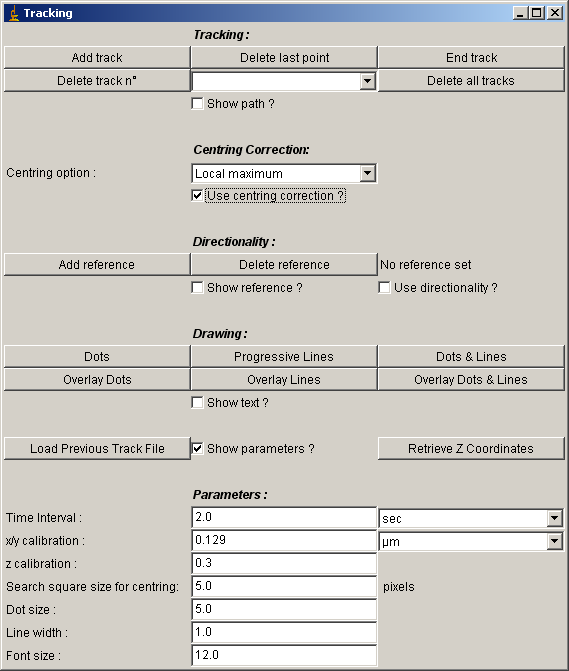
\includegraphics[width=11.298cm,height=13.323cm]{img/CMCIBasicCourse201102-img135.png}
\caption{ Manual Tracker Interface}
\label{fig:img135}
\end{center}
\end{figure}

Then 
\begin{enumerate}
\item Check "centering correction", use Local Maximum.
\item Start manual tracking by clicking "Add track".
\item End tracking by "End Track"
\item Show tracks by "Drawing" Functions"
\end{enumerate}

You could track different particles by repeating steps between 2 and 3. Results window will list the measured positions for particles (Fig. \ref{fig:img137}), and step 4 will show a track overlay image stack (Fig. \ref{fig:img136}).  

%double figure
\begin{figure}[htbp]
\centering
\subfloat[]{\label{fig:img137}
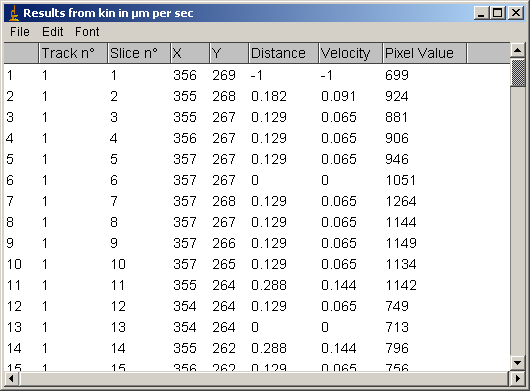
\includegraphics[height=5cm]{img/CMCIBasicCourse201102-img137.png}
}
\subfloat[]{\label{fig:img136}
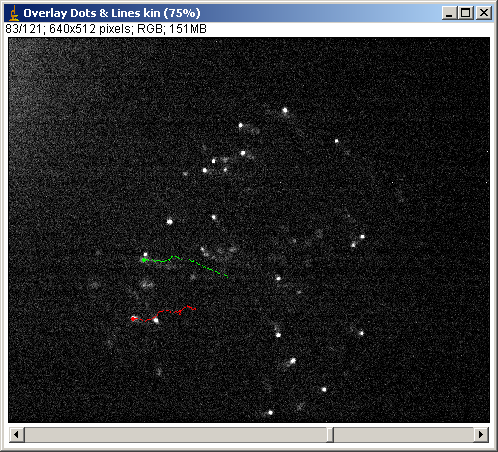
\includegraphics[height=5cm]{img/CMCIBasicCourse201102-img136.png}
}
\caption{ Manual Tracking Results (a) Results table and (b) Track Overlay view.}
\label{fig:ManualTrackResults}
\end{figure} 

Tracked data can be saved by activating "Resut" window and \ijmenu{[File > Save as\dots]}.  \textbf{OPTIONAL:} Copy and paste the result table and plot the track in Excel.
\end{indentexercise}

\subsection{Automatic Tracking}
\label{subsubsec:autotracker}

Automatic tracking reduces the workloads of the researcher, enabling
them to deal with a huge amount of data\footnote{ Texts of this section is mostly from \citep{MiuraME2005}.}. Statistical treatments can
then be more reliable. In addition, the results can be regarded more
objective than manual tracking. Automatic tracking is an optional
function that can be added onto some imaging software. However, these
readily available functions are not adaptable for all analyses since
the characteristics of target objects in biological research vary
greatly. Especially when the target object changes shape over time,
further difficulty arises. For these reasons, automatic tracking often
requires custom programs. In ImageJ, Pascal-like macro programming is
possible and there are many programming functions that enable such
automated segmentation and position measurements.

\subsubsection{CentroidMethod}
The centroid is the average of all pixel coordinates inside the
segmented object and is the most commonly used feature for representing
the object position. The centroid coordinate
$p_{c}(x,y)$ can be calculated as

\begin{equation}
p_{c}(x,y)=(\frac{\sum{x_{i}}}{n_{x}}, \frac{\sum{y_{i}}}{n_{y}})|_{x,y\in\mathfrak{R}}
\end{equation}
%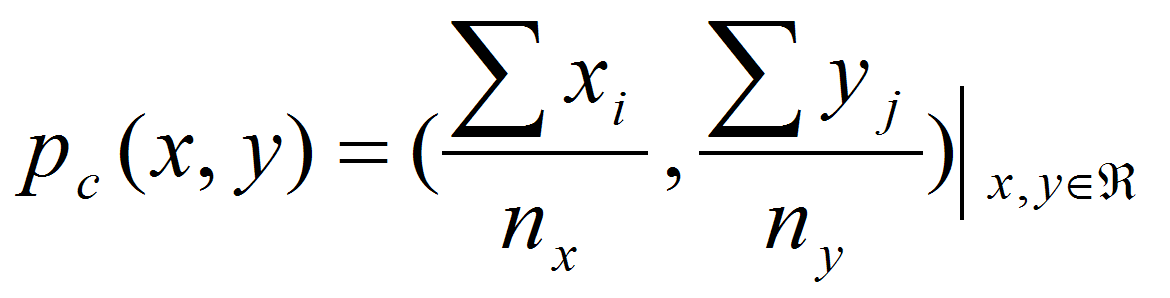
\includegraphics[width=5.398cm,height=1.376cm]{img/CMCIBasicCourse201102-img138.png}

where $\mathfrak{R}$
%
\includegraphics[width=0.459cm,height=0.492cm]{img/CMCIBasicCourse201102-img139.png}
is the region surrounded by the contour, and $n$ is the total
number of pixels within that region. In other words, all x coordinates
of the pixels inside the object are added and averaged. The same
happens for all y coordinates. The derived averages for x and y
coordinates represent the centroid coordinates of the object. The
position of the object can be measured for every frame of the sequence
manually. In ImageJ, centroid calculation is available in the
"Particle Analysis" function.

\subsubsection{Gaussian Fitting Method}

For spherical signals such as fluorescence beads or fluorescently
labeled sub-resolution particle, the signal intensity distribution can
be fitted to a standard two-dimensional Gaussian curve \citep{cmaderson1992, schuetzBJ1997, TardinEJ_2003.pdf}: 

\begin{equation}
I(x,y)=z_{0}+z_{n}\text{exp}\{-\frac{(x-X_{n})^{2}+(y-Y_{n})^{2}}{W_{n}^{2}} \}
\end{equation}
%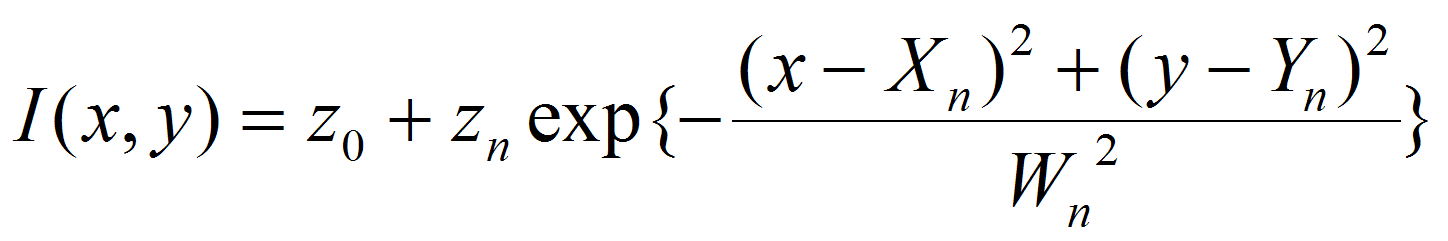
\includegraphics[width=7.62cm,height=1.27cm]{img/CMCIBasicCourse201102-img140.png}
%(5-2)

where $I(x, y)$ is the intensity distribution of an image,
$z_0$ is the background intensity, and
$z_n$ is the height of the peak.
$W_n$ is the width of the curve that
peaks at $(X_n, Y_n)$. This peak position is the signal
position. Although this fitting method is restricted to spherical or
oval objects, it yields the most precise measurements even with a very
low signal-to-noise ratio \citep{cheezumBJ2001}. Another advantage of
the Gaussian fitting method is that the results are in sub-pixel
resolution. Such high resolution can for example enable the analysis of
molecular diffusion in the nm resolution. More discussion on the
localization accuracy in the position measurements can be found in the
literature \citep{oberBJ2004, martinBJ2002, ThompsonBJ2002.pdf}.

\subsubsection{Pattern Matching Method}

In this method, a kernel containing a template pattern of the object is
compared to different positions within the image in order to find a
position with the highest similarity to the kernel. A cross-correlation
function $C(x,y)$ is usually used to evaluate the resemblance of
the template with different parts of the image, (Gilles et al. 1988):

\begin{equation}
\label{eq:simplecorrelation}
C(x,y)=\sum_{i=0}^{n-1}\sum_{j=0}^{m-1}I(x+i)(y+j)\{K(i,j)-\overline{K}\}
\end{equation}
%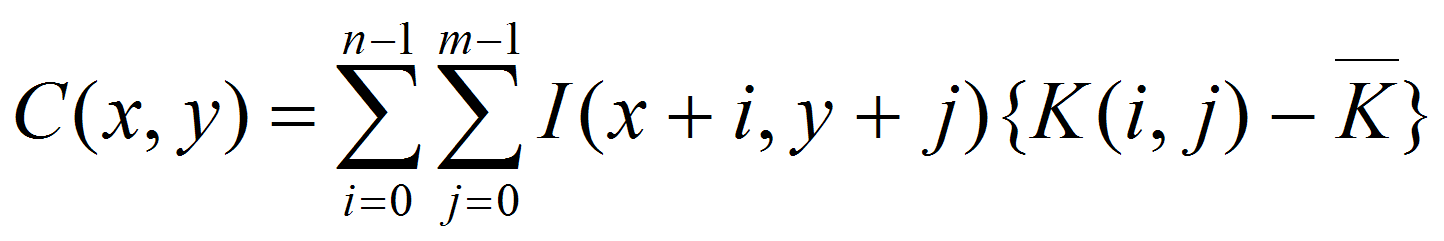
\includegraphics[width=7.373cm,height=1.235cm]{img/CMCIBasicCourse201102-img141.png}
%(5-3)


where $I(x,y)$ is the intensity distribution of the image frame
and $K(i,j)$ is a $n$ x $m$ pixels kernel that
contains the template image pattern. 
%
\includegraphics[width=0.459cm,height=0.564cm]{img/CMCIBasicCourse201102-img142.png}
$\overline{K}$
is the mean intensity of the kernel. $C(x,y)$ will be maximal at
the position where the pattern best matches. In actual application, the
template pattern is sampled in the $k$-th image frame
$I_{k}(x,y)$ by the user manually
or by semi-automatic segmentation. Then the cross-correlation value
$C(x, y)$ between this template kernel and the consecutive
$k+1$-th image frame
$I_{k+1}(x,y)$ can be calculated.
\citet{gellesNAT1988} introduced the following formula for
obtaining the peak position $(x_{c}, y_{c})$:

\begin{equation}
X_{c}=\frac{\sum{x\{C(x,y)-T\}}}{\sum{\{C(x,y)-T\}}}
\end{equation}
%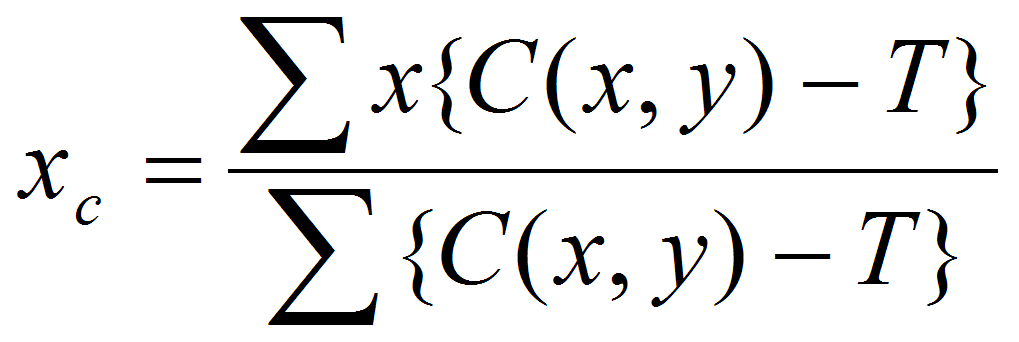
\includegraphics[width=3.986cm,height=1.341cm]{img/CMCIBasicCourse201102-img143.png}
%(5-4)
\begin{equation}
y_{c}=\frac{\sum{y\{C(x,y)-T\}}}{\sum{\{C(x,y)-T\}}}
\end{equation}
%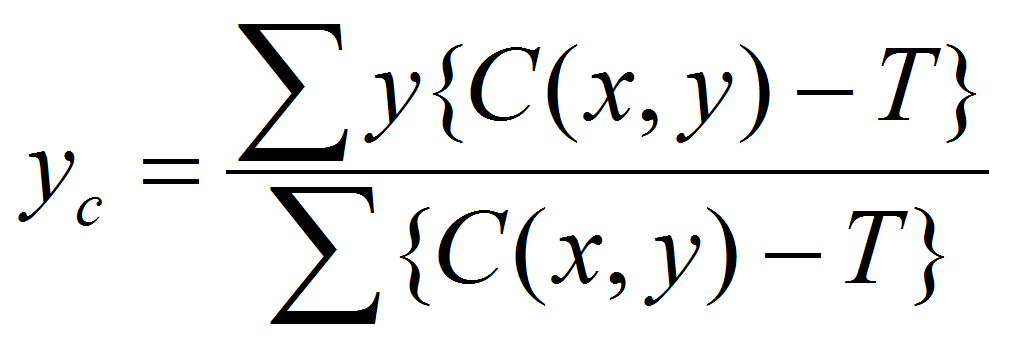
\includegraphics[width=3.951cm,height=1.341cm]{img/CMCIBasicCourse201102-img144.png}
%(5-5)

where $T$ is the threshold value and negative values are
discarded. 
%\textit{(x}\textit{\textsubscript{c}}\textit{,y}\textit{\textsubscript{c}}\textit{)} 
 $(x_{c}, y_{c})$
 corresponds to the centroid of
the magnitude of correlation that is thresholded by $T$. 

Since the cross-correlation function \ref{eq:simplecorrelation} tends to give higher values at
brighter regions rather than at regions of similar shapes, a normalized
form of cross-correlation can also be used:
\begin{equation}
C_{n}(x,y)=\frac{\sum_{i=0}^{n-1}\sum_{j=0}^{m-1}[I(x+i)(y+j)-\overline{I}]\{K(i,j)-\overline{K}\}}{M_{I_{x,y}}\cdot M_{k}}
\end{equation}
%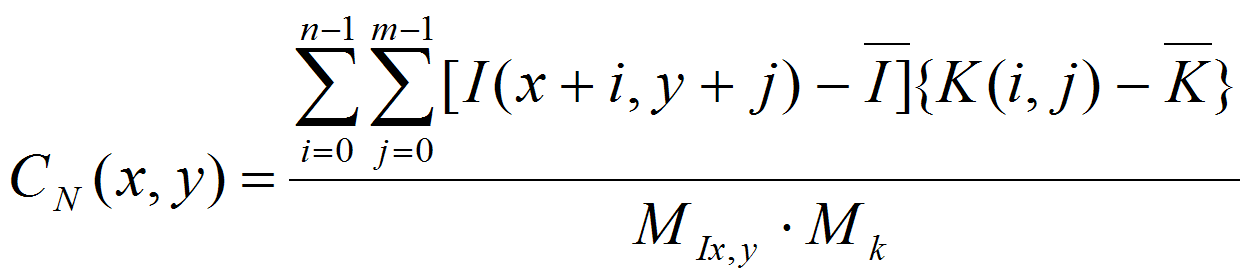
\includegraphics[width=8.573cm,height=1.905cm]{img/CMCIBasicCourse201102-img145.png}
%(5-6)
\begin{equation}
M_{I_{x,y}}=\sqrt{\sum_{i=0}^{n-1}\sum_{j=0}^{m-1}[I_{x+i,y+j}]^{2}}
\end{equation}
%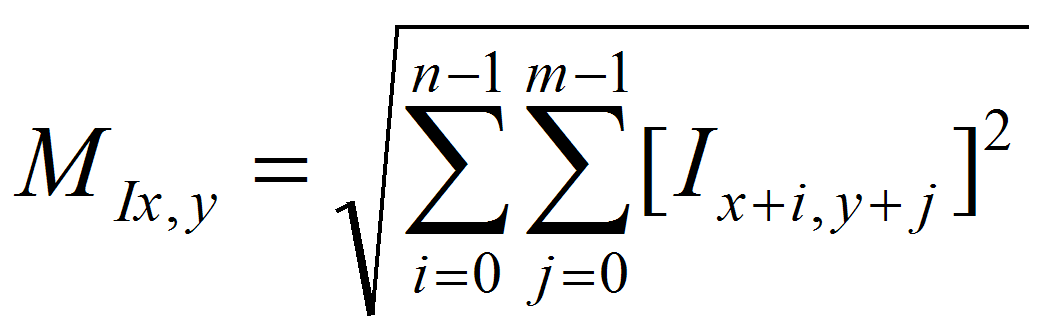
\includegraphics[width=4.339cm,height=1.376cm]{img/CMCIBasicCourse201102-img146.png}
\begin{equation}
M_{k}=\sqrt{\sum_{i=0}^{n-1}\sum_{j=0}^{m-1}[K_{i,j}]^{2}}
\end{equation}
%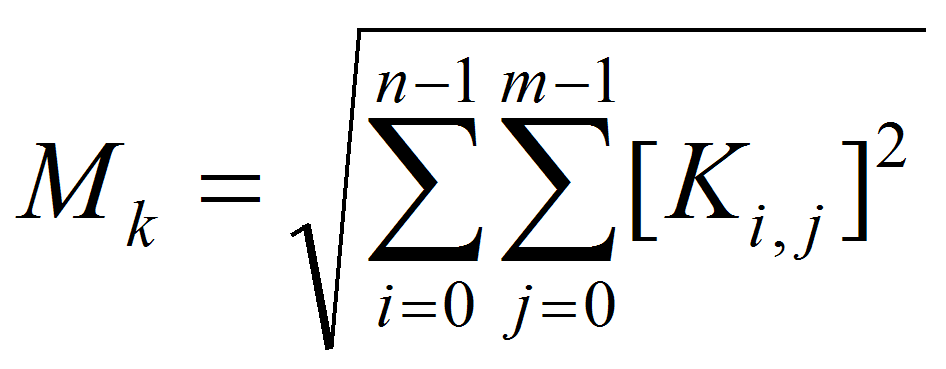
\includegraphics[width=3.528cm,height=1.376cm]{img/CMCIBasicCourse201102-img147.png}

where 
%
\includegraphics[width=0.353cm,height=0.564cm]{img/CMCIBasicCourse201102-img148.png}
$\overline{I}$ is the mean intensity of a portion of the image overlapping the kernel,
and $M_{I_{x,y}}$ and
$M_{k}$ are the root mean square values of
the kernel and the corresponding portion of the image, respectively.
The precision of the measurement is high \citep{cheezumBJ2001}, but
object tracking will fail when the shape of object changes radically
between frames. 

The cross-correlation method has been used extensively in single
particle tracking (SPT). SPT is a technique developed for measuring the
mobility of membrane bound proteins and the movement of motor proteins
with a nanometer precision \citep{gellesNAT1988, Geerts1987, schnappCMOT1988, sheetzNAT1989} and was recently reviewed
\citep{ritchieME2003}. In these studies, a single protein was attached
to a very small gold particle or labeled with a fluorophore and its
movement was analyzed by video microscopy. Theoretical examinations
showed that different modes of protein movement can be discriminated
with nano-meter resolution by measuring the mean square displacement of
the labeled proteins \citep{qianBJ1991}. Various types of membrane
protein motions, such as immobile, directed, confined, tethered, normal
diffusion and anomalous diffusion, were resolved revealing the kinetics
of the membrane protein mobilities \citep{kusumiBJ1993, saxtonBJ1997}.
An automatic tracking program for multiple proteins has been developed
by \citet*{ghoshBJ1994} and was used for measuring the movement of actin patches in Yeast\citep{calssonBJ2002}. 


\subsubsection{ImageJ Tracking Plugins}

Here is a list of object tracking plugins available in ImageJ (Nov. 2006).

\begin{itemize}
\item Particle Tracker
\subitem \url{http://weeman.inf.ethz.ch/particletracker/#general}
\subitem Uses local maxima for estimating particle position, and custom criteria
for discriminating non particles. 

\item MTrack2
\subitem \url{http://valelab.ucsf.edu/~nico/IJplugins/MTrack2.html}

\item MTrackJ
\subitem \url{http://imagescience.bigr.nl//meijering/software/mtrackj/manual.html}
\subitem Initialization should be done manually.

\item Spot Tracker
\subitem \url{http://bigwww.epfl.ch/sage/soft/spottracker/}
\end{itemize}


\begin{indentexercise}{1}
Open image stack \textbf{TransportOfEndosomalVirus.tif}. 
We use "Particle Tracker" for experiencing the automatic tracking \citep{Sbalzarini2005}. 
Refer to "Particle Tracker Tutorials" in the Appendix \ref{app4} and 
examine the difference in the automatic detection and tracking of virus particles 
when different parameters are used.

\end{indentexercise}

\subsection{Summarizing the Tracking data}

Tracking of a moving object results in a list of position coordinates.
This list can be saved as a text file and imported to spreadsheet
software such as Excel. The instantaneous velocity is derived by
calculating the distance between consecutive time points. For example,
if the position of an object at time point $t$ is
$(x_{t}, y_{t})$ and the object moves to a position
$(x_{t+1}, y_{t+1})$ in the next time point
$t + \Delta t$, then the instantaneous velocity $v$ is

\begin{equation}
v = \frac{\sqrt{(x_{t+1} - x_{t})^{2} + (y_{t+1} - y_{t})^{2}}}{\Delta t}
%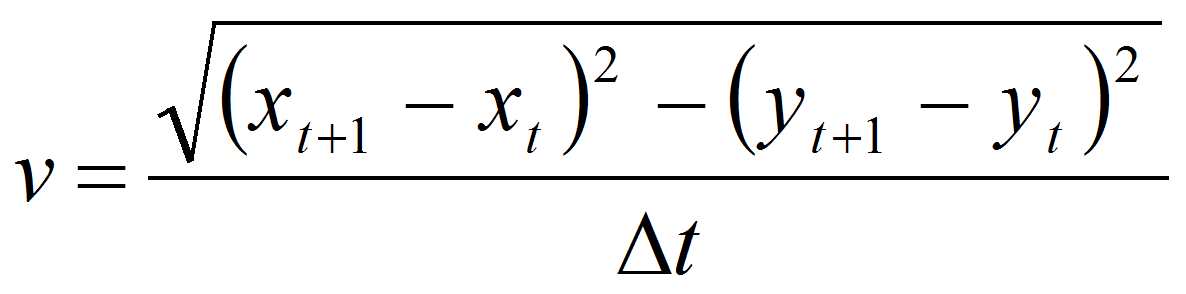
\includegraphics[width=5.398cm,height=1.341cm]{img/CMCIBasicCourse201102-img149.png}
\end{equation}
%(5-7)

For each frame, the instantaneous velocity can be calculated. One way to
summarize the data is to average the resulting instantaneous velocities
and append its standard deviation. In most cases in biology, velocity
changes with time, and this dynamics can be studied by plotting
instantaneous velocity vs. time on a graph. Such plotting reveals
characters of the movement, such as acceleration kinetics or
periodicity.
Movements within organisms can be both random and directed. To make a
clear distinction between these different types of movements, mean
square displacement (MSD) plotting is a powerful method. Although this
method has been extensively used in studying molecular diffusion within
the plasma membrane, it can also be used in other scales such as
bacteria swimming or cell movement within tissue \citep{bergbook1993,SaxtonAnnurevBiophys1997.pdf,kusumiBJ1993, witt2005PLOSB2005,suhADDR2005}.

The most basic equation that describes the diffusion is\footnote{ This equation is for two-dimensional mobility. In case of 3D,
$<r^{2}> = 6D\tau$.} 
\begin{equation}
<r^{2}>= 4D\tau
\end{equation}
%(5-8)

where $r^{2}$ is the mean square
displacement, $D$ is the diffusion coefficient, $\tau$
is the time scale. The MSD is calculated by squaring the net distance a
molecule moved during the period of time $\tau $. For example,
if an object moved from $(0,0)$ to $(x, y)$ during a period of
$\tau $, the square displacement will be

\begin{equation}
r^{2} = x^{2 }+ y^{2 }
\end{equation}
or 
\begin{equation}
r = \sqrt{x^{2 }+ y^{2 }} = \sqrt{4 D \tau}
\end{equation}
%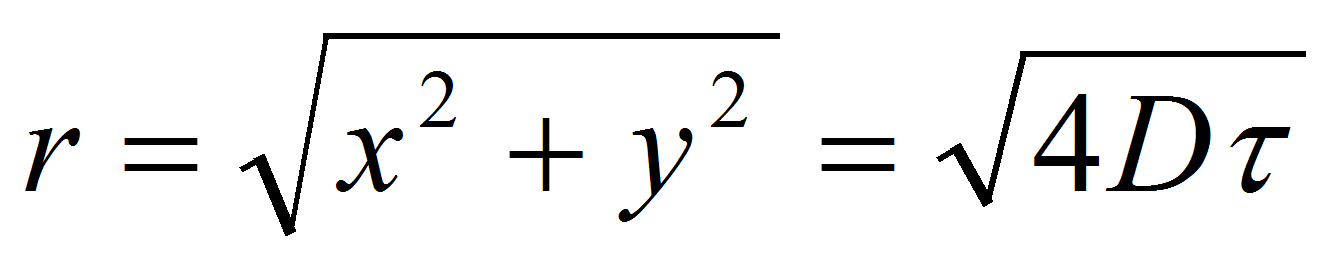
\includegraphics[width=3.951cm,height=0.776cm]{img/CMCIBasicCourse201102-img150.png}
%(5-9)

If we have many samples, then we can average them and the mean square
displacement (MSD) will be

\begin{equation}
\label{eq:2DMSDbasic}
<r^{2}>=<x^{2} + y^{2}>
\end{equation}
%(5-10)

The equation \ref{eq:2DMSDbasic} tells us that the MSD
($r^{2}$) is proportional to
$\tau$, which means that when MSD is plotted against various
$\tau$, the plot will be a straight line with a slope
$4D$ (Fig. \ref{fig:img151} plot a). If the mobility of
the target object is lower, then the slope becomes less steep
(Fig. \ref{fig:img151} plot d).


%figure
\begin{figure}[htbp]
\begin{center}
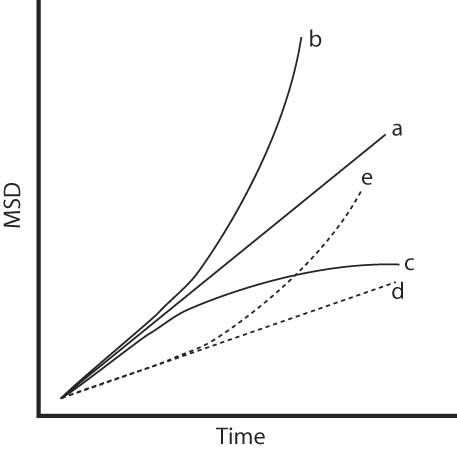
\includegraphics[width=7cm]{img/CMCIBasicCourse201102-img151.jpg}
\caption{ MSD plotting and different types of movement. (a) pure random walk (b) biased random walk (diffusion with drifts) (c)
constrained random walk. (d) pure random walk, but with a lower
diffusion coefficient. In the case of molecules, this could be due to
larger molecule size. In the case of cells, this could be due to a less
migration activity. (e) same as b, but with a lower diffusion
coefficient. }
\label{fig:img151}
\end{center}
\end{figure}
%Figure 1-5-6-1 \ 

The mobility of molecules is not always a pure diffusion. In the case
when there is constant background flow, such as laminar flow in the
medium, molecules drift in a certain direction. This is called
diffusion with drifts, also called "biased
diffusion". Curve b in the Fig. \ref{fig:img151} is a typical MSD
curve of this type. Since the flow causes the movement $vt$,
where $v$ is the flow rate, the displacement $r$ will be


\begin{equation}
r = \sqrt{4 D \tau} + v\tau
\end{equation}
%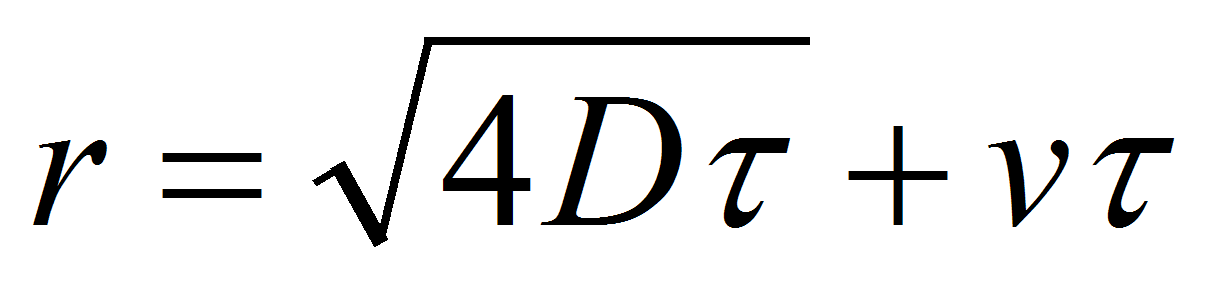
\includegraphics[width=2.646cm,height=0.635cm]{img/CMCIBasicCourse201102-img152.png}
%(5-11)

When MSD $<r^{2}>$is plotted
against time, v$\tau$ causes an upward curvature of the
graph. For example in case of chemotaxis, the direction of movement is
biased towards the chemoattractant source, so that the curve becomes
upward.

Another mode of movement is "constrained
diffusion". This happens when the diffusion is limited
within a space. Consider a molecule diffusing in a bounded space. The
molecule can diffuse normally until it hits the boundary. In such a
case, the MSD curve displays a plateau such that shown in curve c in
Fig. \ref{fig:img151}. When $\tau$ is small, MSD is similar
to the pure diffusion but as $\tau$ becomes larger, MSD
becomes attenuated since the displacement is hindered at a defined
distance. The constrained diffusion is often observed with membrane
proteins \citep{saxtonBJ1997}.




\subsection{ASSIGNMENTS}

{\sffamily\bfseries
Assignments 1-5-5-2: }

Open tubulin dynamics image stack \textbf{kin\_tubulin.stk} and do manual tracking like you did in the exercise \ref{exer:manualtracking}. Track six
points and plot the tracks in a same graph. Is there anything you can
say about their dynamics?\\ 

Images: courtesy of Puck Ohi.